\documentclass{TIJMUjiaoanSY}
\pagestyle{empty}


\begin{document}


%课程名称
\kecheng{Linux系统概论}
%实验名称
\shiyan{实验1\ 在虚拟机中安装并体验Linux}
%教师姓名
\jiaoshi{伊现富}
%职称
\zhicheng{讲师}
%教学日期(格式:XXXX年XX月XX日XX时-XX时)
\riqi{2016年3月2日13:30-15:30}
%授课对象(格式:XXX系XXXX年级XX班(硕/本/专科))
\duixiang{生物医学工程学院2014级生信班(本)}
%实验人数
\renshu{30}
%实验类型
\leixing{验证型}
%实验分组
\fenzu{一人一机}
%学时数
\xueshi{2}
%教材版本
\jiaocai{Linux系统概论上机指南(自编教材)}


%教案首页
\firstHeader
\maketitle
\thispagestyle{empty}

\mudi{
\begin{itemize}
  \item 了解安装Linux的各种方法。
  \item 熟悉常见的Linux发行版。
  \item 掌握VirtualBox的使用方法。
  \item 掌握安装Linux的基本步骤。
  \item 掌握Linux的启动、注销和关机重启。
\end{itemize}
}

\fenpei{
\begin{itemize}
  \item (10')Linux发行版:介绍Linux发行版的含义,罗列常见的Linux发行版,讲解如何选择Linux发行版。
  \item (10')Linux的安装:介绍安装Linux的不同方法,讲解每种方法的优缺点。
  \item (5')虚拟机软件:介绍虚拟机的概念和常用的虚拟机软件。
  \item (75')实验操作:以在VirtualBox中安装Ubuntu和CentOS两个发行版为例,学习VirtualBox的使用,练习Linux的安装。
\end{itemize}
}

\cailiao{
\begin{itemize}
  \item 实验材料:一张Ubuntu 15.04和CentOS 7的安装光盘或ISO映像文件。
  \item 主要仪器:一台安装有Windows操作系统和VirtualBox软件的计算机。
\end{itemize}
}

\zhongdian{
\begin{itemize}
  \item 重点难点:VirtualBox的使用,Linux的安装。
  \item 解决策略:通过演示进行学习,通过练习熟练掌握。
\end{itemize}
}

\sikao{
\begin{itemize}
  \item 列举常见的Linux发行版。
  \item 比较安装Linux各种方法之间的优缺点。
  \item 总结VirtualBox的基本使用方法。
  \item 总结安装Linux的基本步骤。
\end{itemize}
}

\cankao{
\begin{itemize}
  \item Linux基础及应用习题解析与实验指导(第二版),谢蓉\ 编著。中国铁道出版社,2014。
\end{itemize}
}

\firstTail


%教案续页
\newpage
\otherHeader

\noindent
\begin{enumerate}
  \item Linux发行版(10分钟)
    \begin{enumerate}
      \item Linux发行版 = Linux内核 + 实用工具 + 编程工具 + GUI
      \item Linux发行版的两大系统
        \begin{itemize}
          \item Red Hat系:RHEL,CentOS,Fedora,SUSE/openSUSE,……
          \item Debian系:Debian,Ubuntu,Linux Mint,Deepin,……
        \end{itemize}
      \item Linux发行版的选择
        \begin{itemize}
\parpic[fr]{
\includegraphics[width=8cm,height=2.8cm]{c1.linux.distribution.02.png}}
          \item 企业环境:RHEL,SUSE,……
          \item 服务器环境:CentOS,openSUSE,……
          \item 桌面环境:Ubuntu,Fedora,Linux Mint,Deepin,Gentoo,……
        \end{itemize}
    \end{enumerate}
  \item Linux的安装(10分钟)
    \begin{enumerate}
      \item Live CD:一个可引导的CD-ROM,包含运行一个完整操作系统所需的所有内容。可读,不可写。
      \item Live USB:类似于Live CD,但可以更改设置、保存文件、安装软件。
      \item 硬盘安装
	\begin{itemize}
	  \item Wubi(基于Windows的安装程序,Windows-based Ubuntu Installer),DeepWin:无需对硬盘进行格式化或重新分区。简单便利,可惜已经停止维护和更新。
	  \item 虚拟机:在实体计算机上,使用宿主机的硬件资源,通过软件模拟出一台或者多台虚拟计算机,拥有真实计算机的绝大多数功能。安全简便,性能有限。
	  \item 多重引导系统:在计算机上安装不止一个操作系统,但一次只能运行一个操作系统,切换时需要重新启动计算机。安装有风险,使用不方便。
	  \item 单系统:在计算机上只安装一个操作系统。
	\end{itemize}
    \end{enumerate}
  \item 虚拟机软件(5分钟)
    \begin{enumerate}
\parpic[fr]{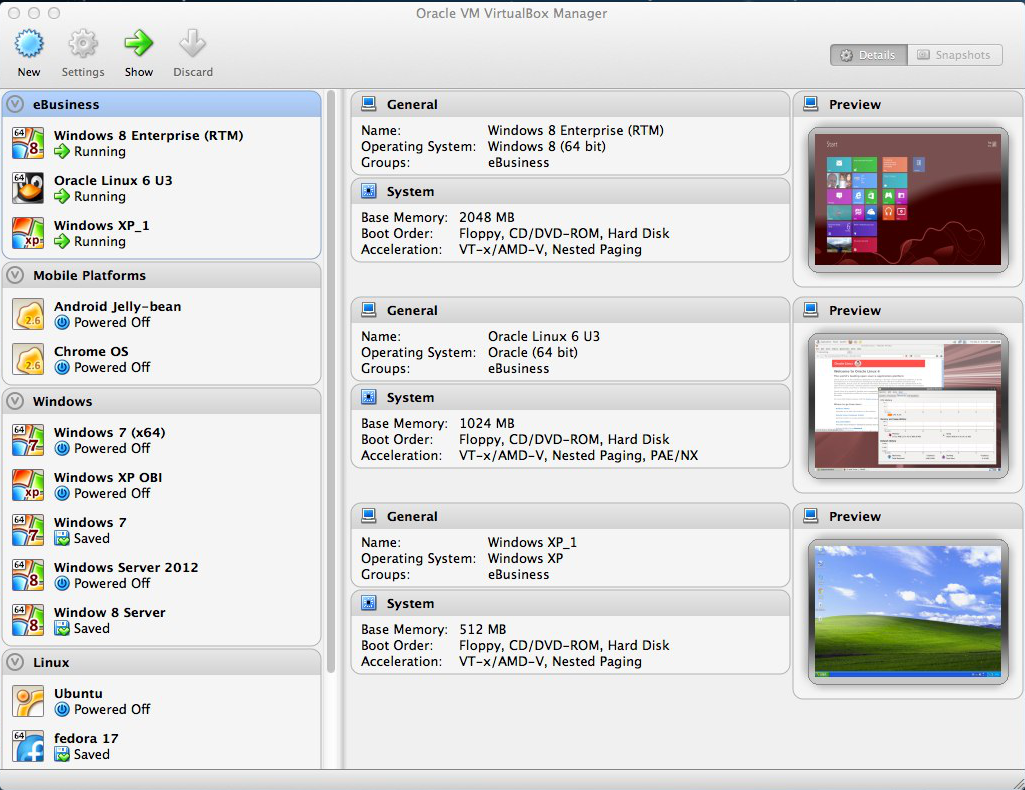
\includegraphics[width=8cm]{c1.virtualbox.01.png}}
      \item 虚拟机:不是一台真正的计算机,而是利用真正计算机的部分硬件资源,通过虚拟机软件模拟出一台计算机。用户可以对虚拟机进行磁盘分区、格式化、安装操作系统等操作,而对本身的计算机没有任何影响。
      \item 虚拟机软件
	\begin{itemize}
	  \item VMware公司出品的相关产品
	  \item 甲骨文公司出品的Oracle VirtualBox
	    \begin{itemize}
	      \item GPL协议,自由软件
	      \item 跨平台(Windows,Linux,……)
	    \end{itemize}
	  \item 微软公司出品的Virtal PC
	\end{itemize}
    \end{enumerate}
  \item 实验操作(75分钟)
    \begin{enumerate}
      \item 在VirtualBox中安装Ubuntu 15.04
	\begin{enumerate}
	  \item 新建虚拟计算机\textcolor{red}{(注意:虚拟电脑的操作系统和版本,内存大小的设置,虚拟硬盘的类型和大小)}
	    \begin{enumerate}
	      \item 启动VirtualBox软件,新建虚拟机
	      \item 选择虚拟电脑的操作系统和版本
	      \item 调整虚拟电脑的内存大小
	      \item 创建虚拟硬盘:选择文件类型、调整硬盘大小、设定存储位置
	    \end{enumerate}


\otherTail
\newpage
\otherHeader


	  \item 在虚拟机中安装Ubuntu 15.04\textcolor{red}{(注意:使用ISO映像的方法,磁盘分区,账户设置)}
	    \begin{enumerate}
	      \item 为虚拟机分配光驱,选择ISO映像
	      \item 启动虚拟电脑
	      \item 选择安装语言,开始安装
	      \item 选择磁盘分区类型
	      \item 设置时区、键盘布局
	      \item 设置个人信息
	      \item 安装系统
	    \end{enumerate}
	  \item 启动Ubuntu 15.04\textcolor{red}{(选择相应的用户,输入对应的密码)}
	  \item 注销用户
	  \item 关机重启
	    \begin{enumerate}
	      \item 图形界面下的操作
	      \item 命令行界面下的操作
	    \end{enumerate}
	\end{enumerate}
      \item 在VirtualBox中安装CentOS 7\textcolor{red}{(参考Ubuntu 15.04的安装过程)}
      \item 在VirtualBox中安装其他的Linux发行版\textcolor{red}{(尝试安装其他的Linux发行版,总结VirtualBox的基本使用方法和Linux安装的基本步骤)}
    \end{enumerate}
\end{enumerate}


\otherTail


\end{document}

